\documentclass{scrartcl}
\usepackage{tikz}
\usetikzlibrary{arrows,automata}
\usepackage{comment}
\begin{document}

% this is a single line comment and wont appear in the final document

% following block within \begin{comment} and \end{comment} are also comments;
\begin{comment}
DFA is defined as below and drawn pictorially

Hints:
- for set symbol, use \{ and \}
- for subscript $q_0$
- $ sets up math mode and you end with $
- also when you use special symbols such as _, ^, | etc, then use \$ to
  bracket them
- if $ doesnt match with another $, you will get warnings
- for math symbols, use \delta, \sum, \epsilon etc.
- for more symbols see http://www.artofproblemsolving.com/wiki/index.php?title=LaTeX:Symbols
- use \\ to denote new line
- for defining table, 
  - ||c c c|| defines 3 columns and so on
  - each row values are separated by &
  - use \space if you want to omit a column
- for drawing the DFA, we use tikz package
  - first 3 lines define the states, which one is initial, final etc
  - far right (eg. {$q_1$} will be drawn in the diagram within the circle
  - q1, q2, etc are like local variables used to define the machine
    and the transitions
  - you can specify how you want the arrows to look like--experiment
\end{comment}

Below is the DFA $M_1$ defined on Page 36 of the ITC \\
textbook. 

% begin math mode with leading \$
$
Q = \{q_0, q_1, q_2 \} 				\\
\sum = \{0, 1 \} 					\\
F = \{q_2 \} 						\\
q_0 = q_1 							\\
\delta = \{ 	((q_0, 0), q_1), 
				((q_0, 1), q_0), 
				((q_1, 0), q_2), 
				((q_1, 1), q_1) \} 	\\
$
% end math mode with trailing \$

Transition Function in Table form: \\

% DFA Table representation

\begin{center}
 \begin{tabular}{||c c c||} 
 \hline
 \space & 0 & 1  			\\ [0.5ex]
 \hline
 $q_1$ & $q_2$ & $q_3$ 		\\
 \hline
 $q_2$ & $q_3$ & $q_2$		\\
 \hline
 $q_3$ & $q_2$ & $q_2$		\\
 \hline
\end{tabular}
\end{center}

DFA in Pictorial form: \\

% DFA pictorial representation

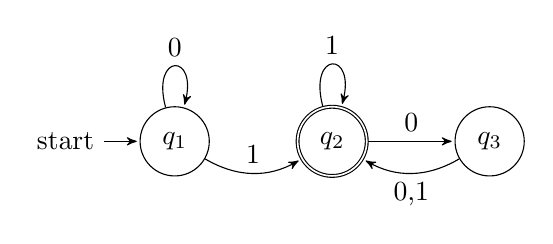
\begin{tikzpicture}[>=stealth',shorten >=1pt,auto,node distance=2cm]
% define the states in the machine
  \node[initial,state	] 	(q1)      				{$q_1$};
  \node[state,accepting]  	(q2) [right of=q1]  	{$q_2$};
  \node[state]         		(q3) [right of=q2]  	{$q_3$};

% define the links
  \path[->] (q1)  edge [loop above] 	node {0} 	(q1)
             edge [bend right]         node {1} 	(q2)
        (q2) edge [loop above]  		node {1} 	(q3)
             edge 				  		node {0} 	(q3)
        (q3) edge [bend left]  		node {0,1} 	(q2);
\end{tikzpicture}
\end{document}
